\section{Methods: The MINI pipeline}

\begin{figure}[h]
    \centering
    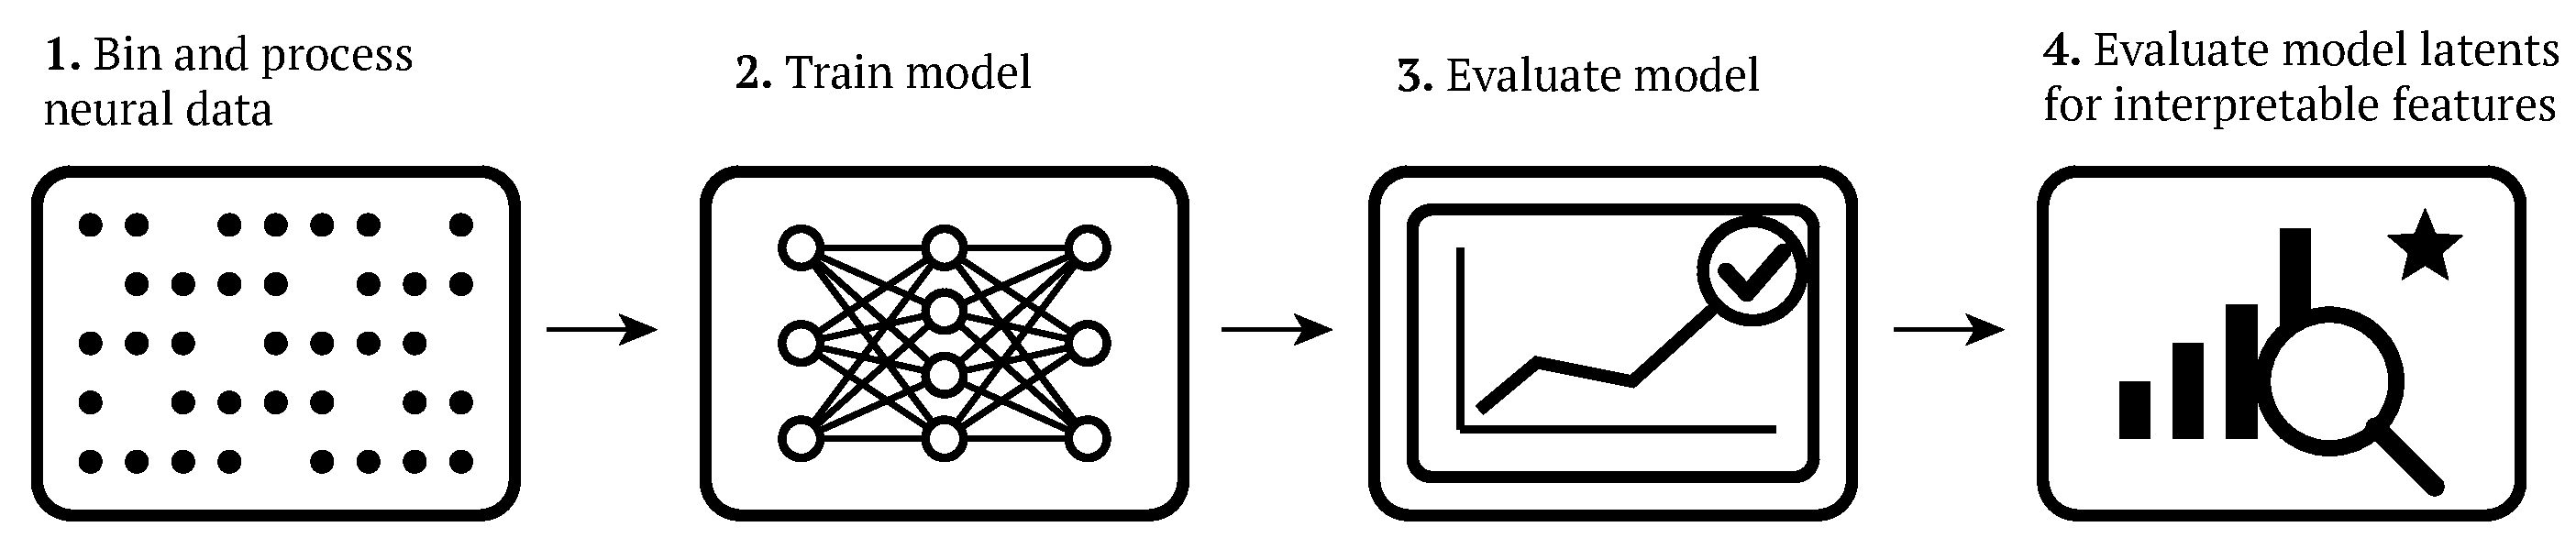
\includegraphics[width=\linewidth]{figures/mini_pipeline.pdf}
    \caption{
        \textbf{The MINI pipeline.} \\
        \small The MINI pipeline is comprised of 4 stages: 1) Spatiotemporal binning and processing of neural data; 2) Training a model; 3) Evaluating a model holistically; 4) Evaluating latents for feature interpretability. Steps 1-3 can be either semi- or fully-automated.
    }
    \label{figure:mini_pipeline}
\end{figure}

The MINI pipeline transforms high-dimensional neural data into a set of interpretable latents in four primary stages (\autoref{figure:mini_pipeline}), the first three of which can be fully automated.

\subsection{Data preprocessing}

The pipeline's first stage prepares neural data for model training. MINI includes utilities to process outputs from common spikesorters (e.g. Kilosort ~\cite{pachitariu_2016_kilosort}) by aggregating, binning, and normalizing spike times into a 2D matrix of time by space, in which each bin contains neural activity from a neural unit for a specific time period. Normalization operations include min-max and z-scoring, applied across either the spatial or temporal dimension. This processing is readily adaptable to other forms of acquired neural data, such as ROIs from calcium imaging data processed by tools like Suite2p ~\cite{pachitariu_2017_suite2p}. Alternatively, users may pass their own preprocessed neural data directly to the model training stage.

\begin{figure}[tbph]
    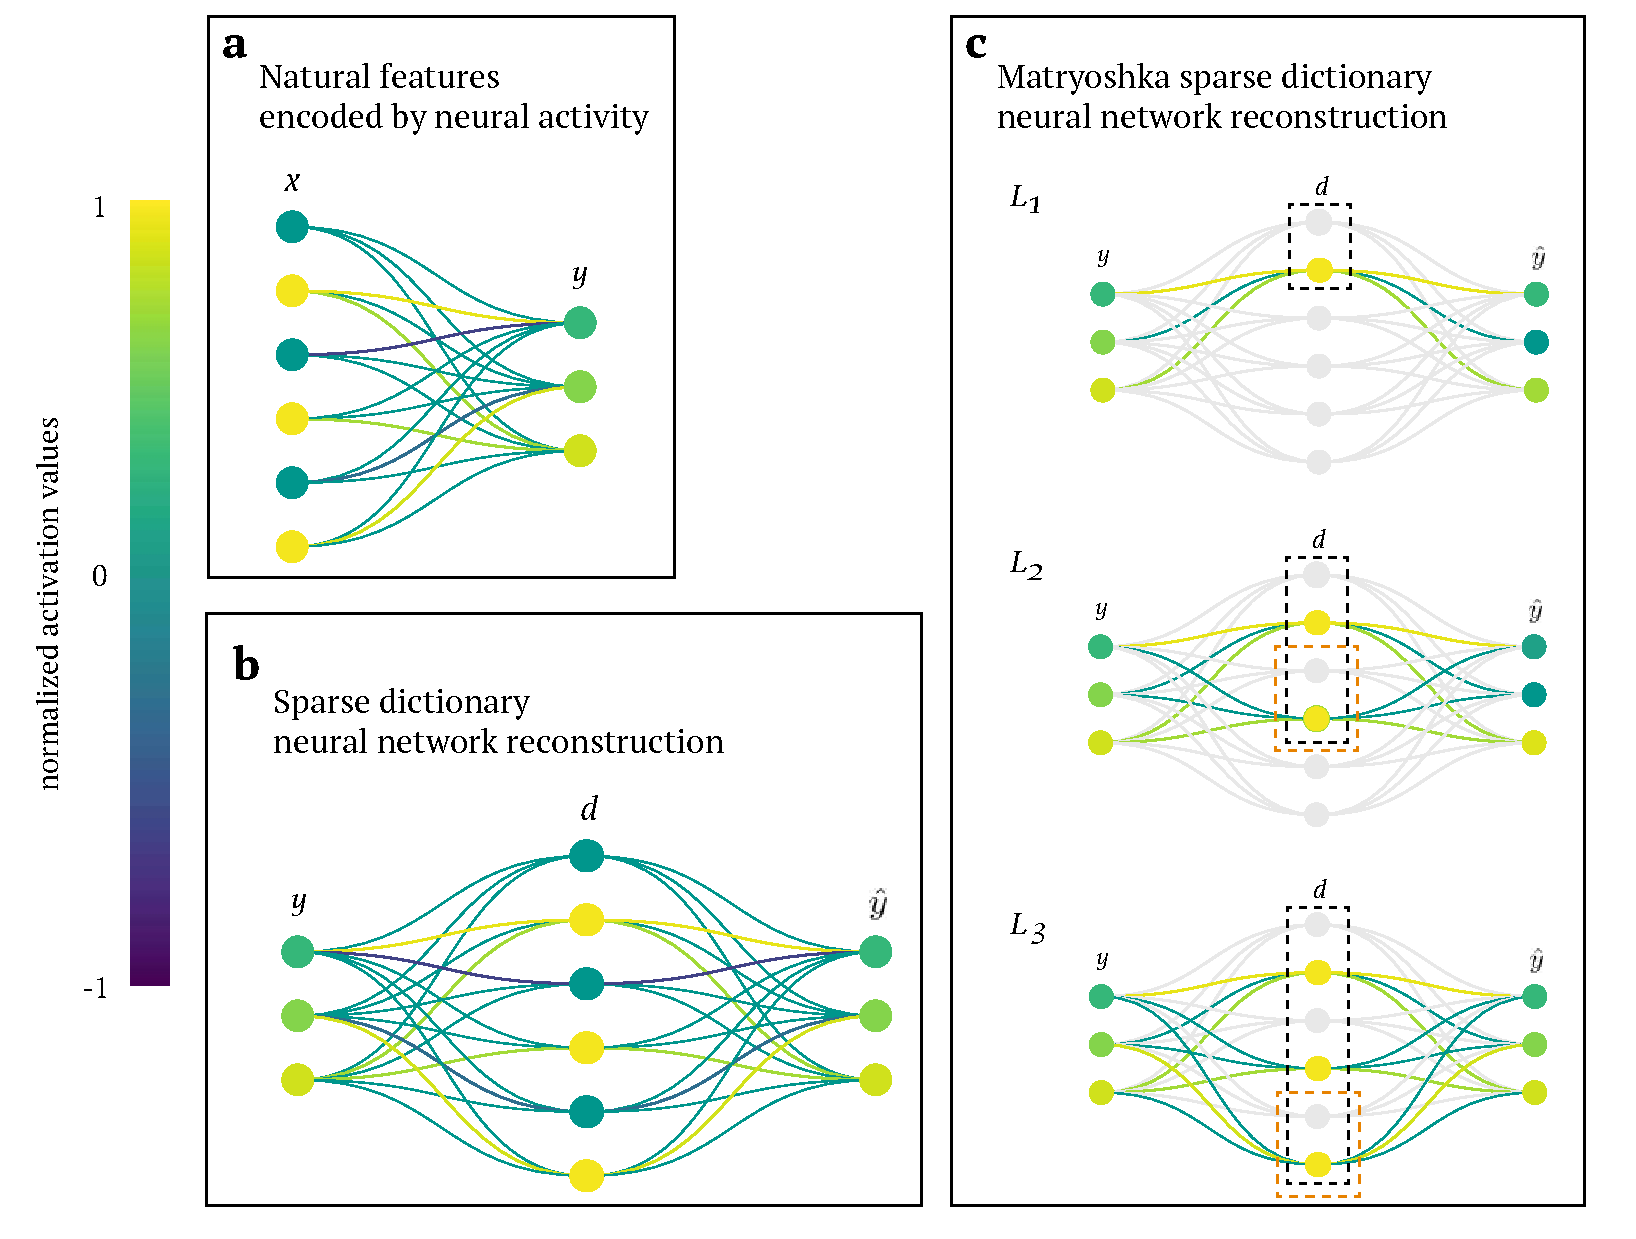
\includegraphics[width=\linewidth]{figures/sdnn_arch.pdf}
    \caption{
        \textbf{Model architecture considerations} \\
        \small
        (\textbf{a}) Natural, "real-world" features $x$ are encoded by neural activity $y$. In this example, three active features are simultaneously represented by the joint activity of three neurons. (\textbf{b}) A SDNN reconstructs neural activity $z$ based on $y$ via sparse dictionary elements $d$. When training is successful, $d$ corresponds to $x$: sparse dictionary elements (i.e. model neurons) represent natural features. If $z$ tries to recreate $y$ exactly ($\hat{y}$), the model is an autoencoder; in other scenarios (e.g. $z$ is separate but dependent on or related to $y$) it is a transcoder or crosscoder. (\textbf{c}) A Matryoshka SDNN segments the latent space into multiple levels, each of which attempts to do a full reconstruction of the target neural activity. The black boxes indicate the latents involved in a single level, while the light-red boxes indicate the additional latents used at lower-levels. A $k$=1 value is chosen for top-$k$ selection of latents to recruit for reconstruction at each level (the yellow neuron within each light-red box). Latents in the highest-level ($L_1$) will often correspond to high-level features (e.g. a round object), while latents exclusive to the lowest-level ($L_3$) will often correspond to low-level features (e.g. a basketball). (\textbf{d}) Incorporation of a transformer block with sequence input allows imbuing the latent space with temporal information corresponding to the evolution of the sequence, which can lead to improved reconstruction and interpretability. In parallel, each sample in the input sequence is transformed by the same encoding dictionary matrix to yield a latent space sequence. Causal self-attention is then performed on this sequence of latents via a single, small multi-head transformer block, yielding a final latent space. The latents are sparsified via top-k and transformed by the decoding dictionary matrix to yield the neural data reconstruction, as in the single, non-sequential input case. 
    }
    \label{figure:sdnn_arch}
\end{figure}

\subsection{Model training}

In stage 2, a SDNN model is trained to reconstruct the processed neural data from latent, sparsely active dictionary elements -- the model's hidden layer neurons\footnote{In a SDNN model: model neuron = dictionary element = latent}. The end goal is for these latents to represent disentangled, interpretable representations\footnote{In our vernacular: interpretable latent $\approx$ feature $\approx$ representation} encoded by the neural activity (\autoref{figure:sdnn_arch}a,b). Sparsity encourages the model to discover a monosemantic dictionary, in which each latent corresponds to a single feature. For instance, a latent from a model trained on visual cortex activity may correspond to a particular property of a visual stimulus, while a latent from a model trained on motor cortex activity may correspond to a specific aspect of movement.

The model can take three forms ~\cite{lindsey_2024_crosscoders}, depending on the relationship between the input and target neural data:
\begin{itemize}[nosep, leftmargin=1em, topsep=-0.5em]
    \item \textbf{Autoencoder}: The model reconstructs its own input; e.g. V1 activity based on V1 activity.
    \item \textbf{Transcoder}: The model reconstructs a dependent target of its input; e.g. V2 activity based on V1 activity.
    \item \textbf{Crosscoder}: The model reconstructs a related target of its input; e.g. V1 activity on day 2 based on V1 activity on day 1.
\end{itemize}
In all cases, the model is trained to minimize the difference between the reconstructed and actual target neural data. The full training procedure is summarized in \nameref{algorithm:sdnn_model_training}. Three key components are particularly worth noting: the batch top-$k$ sparsity, Matryoshka architecture, and integration over latent space history via self-attention.

A batch top-$k$ operator preserves only the $k \cdot B$ latents with the highest activation magnitudes across a batch of size $B$. This approach directly controls sparsity in contrast to indirect approaches (e.g. an L1 penalty) and flexibly permits the number of active features to vary per sample in the batch, aligning with the variable complexity of neural states. A novel variant of the Matryoshka SDNN architecture ~\cite{bussmann_2025_msae} segments the latent space into hierarchical levels, where each level attempts a full reconstruction of the target neural activity (\autoref{figure:sdnn_arch}c). This allows for multi-scale feature representation at single timepoints, and mitigates "feature absorption," a common issue where general features subsume specific ones ~\cite{chanin_2024_feature_absorption}. For example, a model can learn that a "drifting grating" is a subset of the more general "grating" visual stimulus class without sacrificing the representation of either (\nameref{subsubsection:allen_dataset_results}). Lastly, if input data is provided as a sequence of timebins rather than single timebins, an optional transformer block can integrate information over the latent space history via self-attention (\autoref{figure:sdnn_arch}d), enabling the model to learn features corresponding to evolving temporal dynamics, rather than just instantaneous neural patterns. 

The combination of these architectural options creates a flexible but large search space for model design. Searching this space effectively is crucial, as we empirically find that these components can significantly improve both reconstruction accuracy and feature interpretability (\nameref{subsubsection:architecture_details}). To streamline this search with minimal manual specification, MINI supports fully automated training via hyperparameter sweep configurations that support local or distributed training across one or multiple CPUs or GPUs (\nameref{subsubsection:hyperparameter_sweeps}).

\subsection{Model evaluation}

In stage 3, the trained model is evaluated using a variety of metrics to assess its performance. 

(SAEBench ~\cite{karvonen_2025_saebench})

\begin{itemize}
    \item (We implement all metrics from SAEBench which are not language-model specific, plus a couple of our own)
    \item L0 of latents
    \item R\textsuperscript{2} (var explained) and cos sim of reconstruction-to-actual neural activity for each spatial bin, and each temporal bin
    \item Latent density histogram (as in SAEBench)
    \item Variance explained of overall reconstruction from each latent (variance shouldn't be in just a few features) ?
    \item Spectral frequency analysis to ensure temporal frequency content is preserved?
\end{itemize}

\begin{figure}[h]
    \centering
    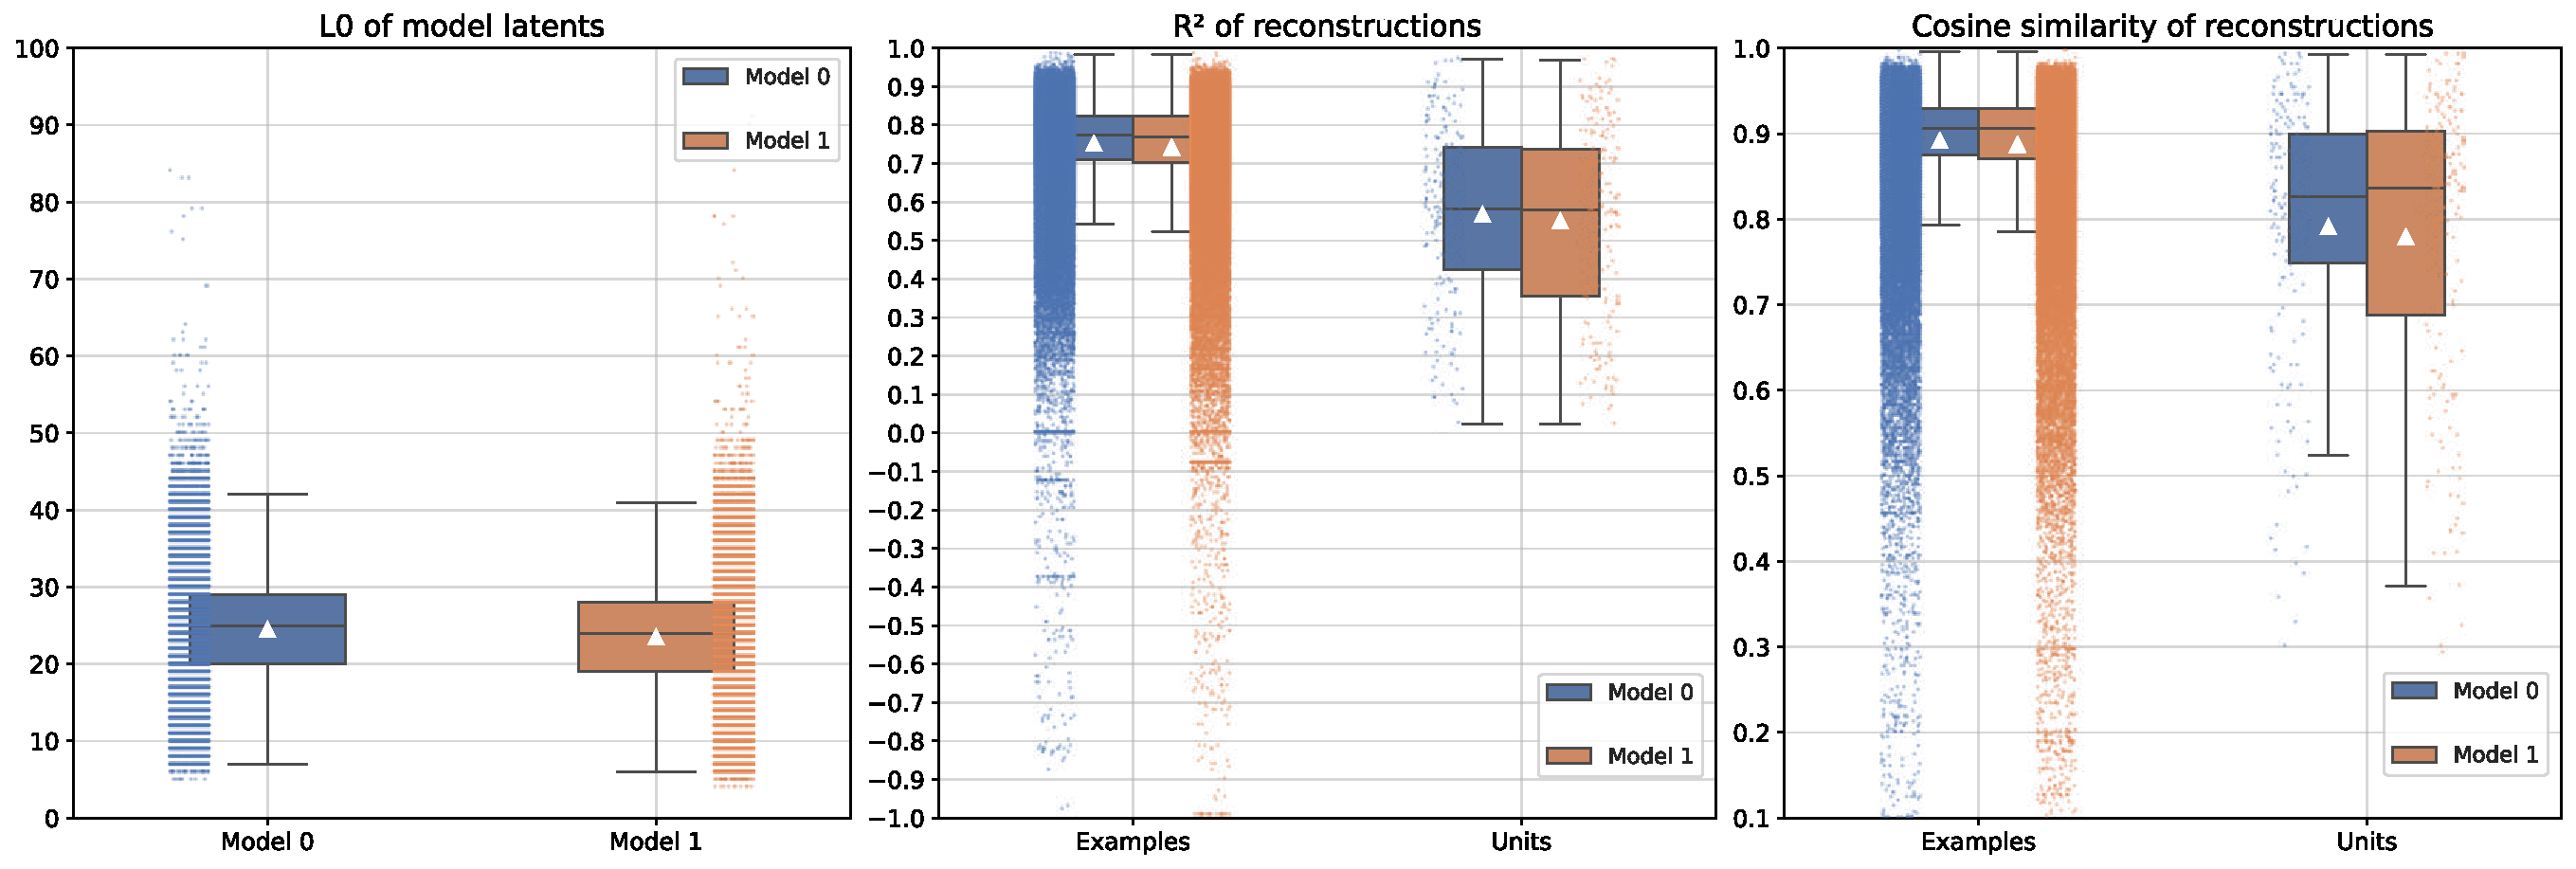
\includegraphics[width=\linewidth]{figures/model_eval.pdf}
    \caption{
        \textbf{Model evaluation metrics.} \\
        \small By default, trained models are evaluated via the following metrics: latent L0 (left), and R\textsuperscript{2} (middle) and cosine similarity (right) of reconstruction-to-actual neural activity for each temporal ("Examples") and spatial ("Units") bin. ... Additional features, such as the R\textsuperscript{2}of overall neural data reconstruction for each individual latent, can be specifed and included.
    }
    \label{figure:model_eval}
\end{figure}

\subsection{Latents evaluation}

Finally in stage 4, the latents produced by the model are evaluated for interpretability. This can include visualizing their activation patterns over time and experimental conditions, as well as assessing their decoding performance. We detail typical approaches to feature evaluation in \nameref{section:results}.
